
\begin{frame}{NP effect (LMM)}
	\begin{flushright}
		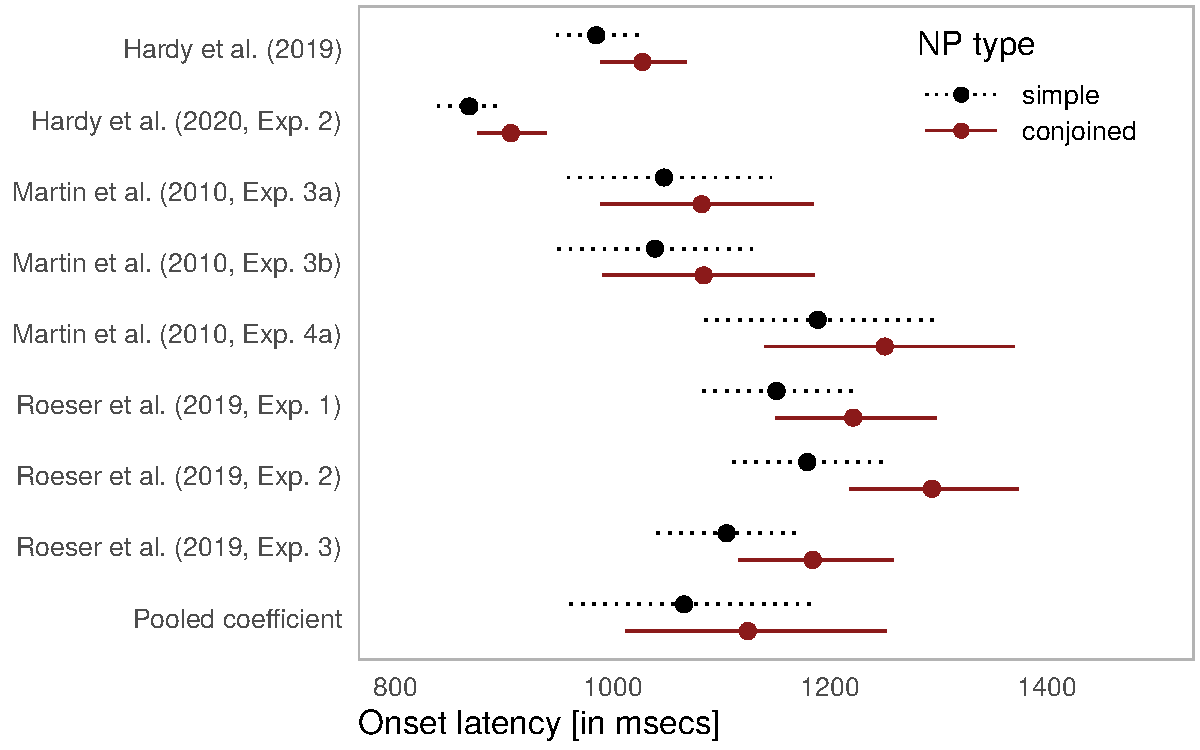
\includegraphics[scale=.5]{NPmeta.pdf}
	\end{flushright}
\end{frame}


\begin{frame}{NP effect (LMM)}
	\begin{flushright}	
		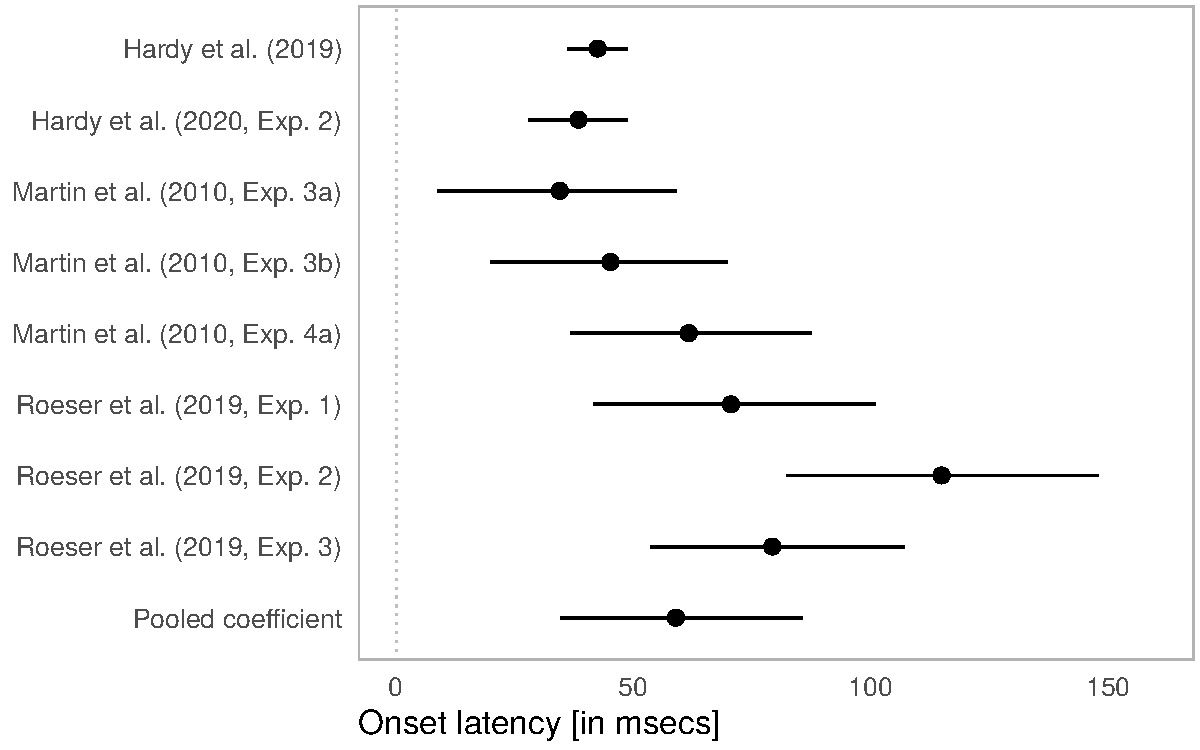
\includegraphics[scale=.5]{NPmetadiff.pdf}
	\end{flushright}
\end{frame}



\begin{frame}{Model comparisons}
\begin{scriptsize}
% latex table generated in R 4.0.2 by xtable 1.8-4 package
% Tue Aug 18 15:17:51 2020
	\begin{table}[ht]
	\centering
	\caption{\scriptsize{Predictive performance estimated as the \textit{expected log pointwise predictive density} ($\widehat{elpd}$) \parencite{vehtari2015pareto, vehtari2017practical}. Models are ordered by predictive performance (model with highest predictive performance in top row)}. Standard error in parentheses.}
		\begin{tabular}{lrrl}
		\toprule
		Models & $\updel\widehat{elpd}$ & $\widehat{elpd}$ & Description \\ [1ex]
		\midrule
		\rowcolor{yellow!40!white}MoG-1 & -- & -201,486 (176) & Mixing proportions by NP \\ [1ex]
  		MoG-0 & -15 (8) & -201,500 (176)  & Null model \\ [1ex]
 		\rowcolor{yellow!40!white}LMM-1 & -1,006 (97) & -202,492 (214) & NP effect \\ [1ex]
  		LMM-0 & -1,192 (92) & -202,678 (212) & Null model \\ [1ex]
 		LMM-2 & -3,537 (214) & -205,022 (307) & Unequal variance \\ [1ex]
		\bottomrule
		\end{tabular}\\
		\textit{Note.} LMM = Linear mixed effects model; MoG = Mixture of Gaussians 
	\end{table}
\end{scriptsize}
\end{frame}



\begin{frame}{Probability of long latencies (MoG)}

	\begin{flushright}
		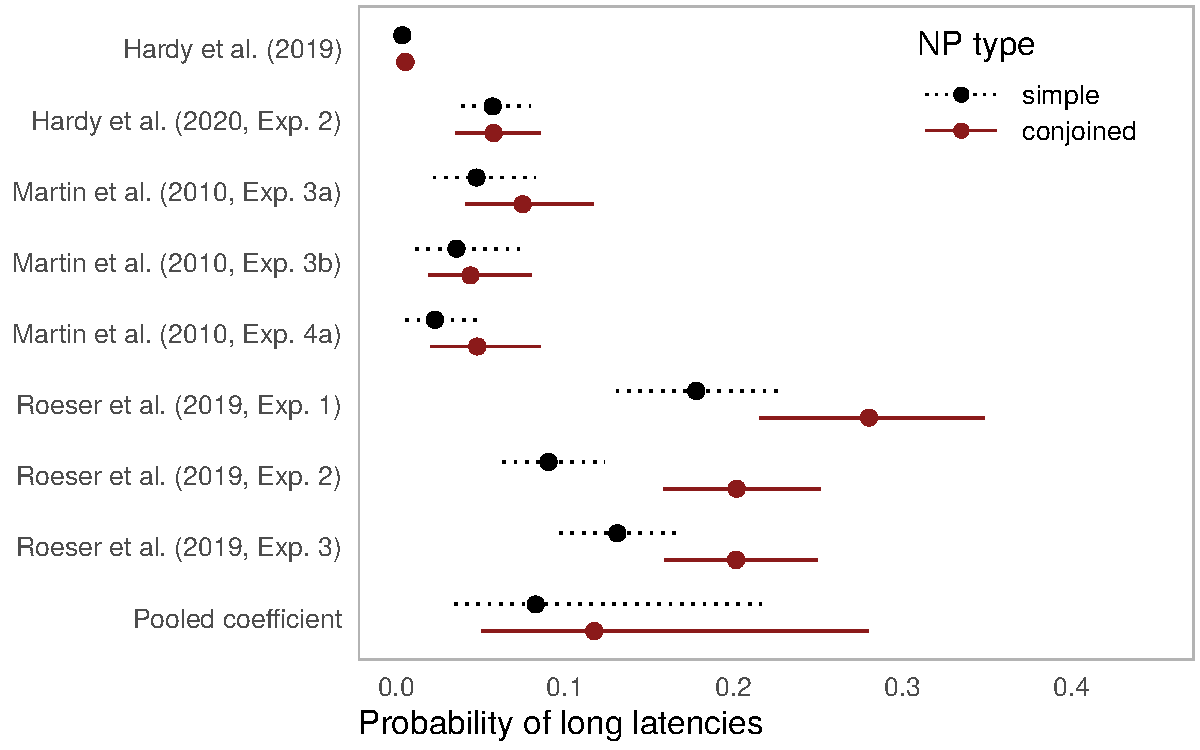
\includegraphics[scale=.5]{mogmeta.pdf}
	\end{flushright}


\end{frame}